

\section{Représentation de documents}

\begin{frame}
\frametitle{Représentation de documents textuels}

Modèle de données basé sur des \alert{graphes}, permettant de représenter des
données régulières ou irrégulières.

\vfill

\alert{Idées de base}

\begin{description}
  \item[Les données sont auto-décrites.] Le contenu vient avec sa propre
  description.
  
 \item[Structures riches.] Le contenu se décrit avec des listes, des
 enregistrements imbriqués, des ensembles.

  \item[Typage flexible.] Les données peuvent être typées (``c'est un entier''),
  et/ou structurées (``cette partie du graphe \alert{doit} avoir telle forme''), et/ou ni l'un ni
  l'autre. Dans ce dernier cas c'est à l'application d'effectuer le contrôle.
 
   \item[Sérialisation.] Structure \alert{et} contenu doivent pouvoir être transformés
      ensemble en une chaîne de caractères autonome.

\end{description}

\end{frame}

\begin{frame}[fragile]
\frametitle{Exemple avec JSON}

Point de départ\,: \alert{listes associatives},  i.e., des
enregistrements avec des paires (clé, valeur).

\begin{verbatim}
{nom: "Alan", tél: 2157786,  email: "agb@abc.com"}
\end{verbatim}

Extension naturelle\,: les valeurs sont elles-mêmes d'autres structures.

\begin{verbatim}
{nom: {prénom: "Alan",  famille: "Black"},
     tél: 2157786,
     email: "agb@abc.com"}
\end{verbatim}

Autre exemple: imbrication de listes.

\begin{verbatim}
    {name: "Alan", téls: [2157786, 2498762] }
\end{verbatim}

NB\,: c'est la version sérialisée, une chaîne stockable sur disque.
\end{frame}

\begin{frame}
\frametitle{Vue conceptuelle: modélisation sous forme arborescente}

Données représentées par des arbres. Les étiquettes sont
sur les arêtes, les valeurs sur les feuilles.



\begin{center}
\footnotesize
\begin{minipage}[t]{5cm}

\includegraphics[width=5cm]{label_on_edges1}
\end{minipage} \qquad
\begin{minipage}[t]{5cm}

\includegraphics[width=5cm]{label_on_edges2}
\end{minipage} 
\end{center}

Base du \alert{raisonnement} pour opérations (de recherche, de navigation, ...)
\end{frame}

\begin{frame}
\frametitle{Autre possibilité\,: avec n{\oe}uds-étiquettes}

On peut représenter à la fois les étiquettes et les valeurs 
comme des n{\oe}uds.

\medskip


\includegraphics[width=\textwidth]{simple_xml_tree}

\medskip

\begin{remark}
Choix de représentation du langage XML. 
\end{remark}

\end{frame}

\begin{frame}[fragile]
\frametitle{Plus puissant que la représentation relationnelle?}

Oui, car facile de représenter des données régulières:

\begin{tinyverbatim}
 { person:  {name: "alan", phone: 3127786, email: "alan@abc.com"},
   person:  {name: "sara", phone: 2136877, email: "sara@xyz.edu"},
   person:  {name: "fred", phone: 7786312, email: "fd@ac.uk"} } 
\end{tinyverbatim}

\begin{remark}
\begin{itemize}
\item on peut représenter des données régulières
\item probablement pas du tout efficace dans ce dernier cas.
\end{itemize}
\end{remark}

$\Rightarrow$ peut être utile pour échanger des informations\,; pas pour les
stocker nativement.
\end{frame}

\begin{frame}[fragile]
\frametitle{Plus intéressant: flexibilité de la représentation}

Quel degré de varation accepte-t-on dans une base documentaire (données manquantes, doublons, 
structures variables, etc.)?

\vfill
Exemple extrême,\:

\begin{tinyverbatim}
 {person: {name: "alan", phone: 3127786, email: "agg@abc.com"},
  person: &314
          {name: {first: "Sara", last: "Green"               },
           phone: 2136877, 
           email: "sara@math.xyz.edu",
           spouse: &443                                      },
  person: &443
          {name: "fred", Phone: 7786312,  Height: 183,
           spouse: &314                                      }}
\end{tinyverbatim}

\begin{beamerboxesrounded}{Identité des n{\oe}uds}
En se donnant le moyen d'identitifer des n{\oe}uds, on peut y faire
référence, et décrire des cycles et des modèles objet.
\end{beamerboxesrounded}
\end{frame}

\subsection{Deux langages de représentation -- XML et JSON}

\begin{frame}
\frametitle{XML: données ``semi-structurées''}

XML est d'abord un standard du World-Wide-Web Consortium (W3C).

\begin{itemize}
  \item La sérialisation de documents XML est normalisée, ce qui permet
       des échanges réseau sans perte d'information.
 
  \item XML est un format générique, qui se spécialise ensuite en
     \alert{``dialectes''} pour des domaines spécificque (e.g., XHTML,
     affichage dans un navigateur).

  \item Le W3C a défini des standards associés: DOM (le ``modèle''), 
   XSchema (le typage), XPath (navigation), XSLT (restructuration),
     XQuery (requêtes), et beaucoup d'autres.
\end{itemize}

\begin{remark}
\begin{description}
\item[1.]
XML est une version simplifiée de \alert{SGML}.
\item[2.]
HTML, jusqu'à la version 4.0, est \alert{aussi} une variante de SGML. XHTML
est un dialecte XML.
\end{description}
\end{remark}

\end{frame}


\begin{frame}
\frametitle{Documents XML: modèle et sérialisation}

\begin{description}

\item [Modèle] Un document XML est un arbre, chaque n{\oe}ud a un type particulier.

\item [Sérialisation] tout document XML peut être transformé en une chaîne
   de caractères représentant l'arobrescence du document.
 each node.

\end{description}

La norme XML définit une \alert{syntaxe}. Aucune interprétation n'est
définie à priori.

\vfill

Les dialectes XML imposent des contraintes, et définissent une interprétation.


\begin{beamerboxesrounded}{Le dialecte XHTML}
Un document XHTML est un document XML. Il obéit à des contraintes de structure, et s'interprète
sous forme de règles d'affichage à l'écran.
\end{beamerboxesrounded}

\end{frame}

\begin{frame}
\frametitle{Modèle: un document est un arbre}

Une application manipule un document XML comme un arbre.

%\scalebox{.8}{
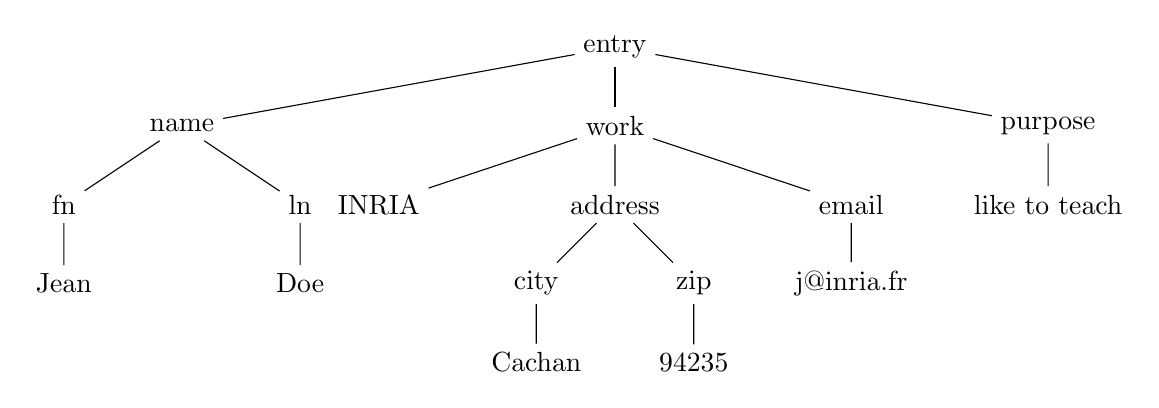
\begin{tikzpicture}
[level distance=10mm,
every node/.style={inner sep=3pt},
level 1/.style={sibling distance=55mm},
level 2/.style={sibling distance=30mm},
level 3/.style={sibling distance=20mm}]
\node {entry}
	child {node {name}	
		child {node  {fn}
			child {node {Jean}}
		}
		child {node {ln}
			child {node  {Doe}}
			}
	}
	child {node {work}
			child {node {INRIA}}
			child {node {address}
				child {node {city}
				  child {node{Cachan}}
					}
				child {node {zip}
				  child{node{94235}}
				}
			}
			child {node {email}
			  child{node{j@inria.fr}}
			}			
	}
		child{node{purpose}
		  child {node{like to teach}}
	};
\end{tikzpicture}}

Exemple: interfaces de programmation (DOM); langages de navigation (XPath),
restructuration (XSLT), recherche (XQuery)
\begin{remark}
Une exception: l'API SAX s'applique à la forme sérialisée d'un document XML.
\end{remark}

\end{frame}

\begin{frame}[fragile]
\frametitle{Forme sérialisée}

Exemple\,:

\begin{tinyverbatim}
<entry><name><fn>Jean</fn><ln>Doe</ln></name>INRIA<adress><city>
Cachan</city><zip>94235</zip></adress><email>j@inria.fr</email>
</job><purpose>like to teach</purpose></entry>
\end{tinyverbatim}
avec une petite mise en forme\,:
\begin{tinyverbatim}
<entry>
   <name>
      <fn>Jean</fn>
      <ln>Doe</ln> </name>
   <work>
      INRIA
      <adress>
         <city>Cachan</city>
         <zip>94235</zip> </adress>
      <email>j@inria.fr</email> </work>
   <purpose>like to teach</purpose>
</entry>
\end{tinyverbatim}
\end{frame}

\begin{frame}[fragile]
\frametitle{XML permet de structurer des documents textuels}

Un document textuel difficile à interpréter pour un logiciel.
\begin{tinyverbatim}
The book ``Fundations of Databases'', written by Serge Abiteboul,
Rick Hull and Victor Vianu, published in 1995 by Addison-Wesley
\end{tinyverbatim}
Avec structuration XML\;:
\begin{tinyverbatim}
<bibliography>
  <book>    
    <title> Foundations of Databases </title>
    <author> Abiteboul </author> 
    <author> Hull </author> 
    <author> Vianu </author>
    <publisher> Addison Wesley </publisher> 
    <year> 1995 </year> </book>
  <book>...</book>
</bibliography>
\end{tinyverbatim}

Une  application peut construire l'arbre XML, en extraire des parties, 
renommer, restructurer, recherche selon certains critères, etc. 
\end{frame}

\begin{frame}[fragile]
\frametitle{Qui utilise XML?}

XML est LE standard pour la représentation  de données textuelles.

\vfill
\alert{Exemples}\,: XHTML, DocBook, RSS, ...

\vfill

XML est AUSSI utilisé pour sérialiser des données applicatives, par exemple pour les données
gérées par vos applications personnelles.


\vfill

\alert{Exemples}\,: Traitements de texte (Word), tableurs (Excel), calendriers, graphiques (en SVG), etc.

\vfill

\begin{beamerboxesrounded}{Dans tous les cas}
La représentation en XML permet de \alert{réutiliser} le contenu, de l'échanger avec d'autres applications.
\end{beamerboxesrounded}
\end{frame}

\begin{frame}[fragile]

\begin{lstlisting}[language=myXML]
<?xml version="1.0" encoding="UTF-8" ?>

<rss version="2.0">
<channel>
	<title>Webdam Project</title>
	<atom:link href="http://webdam.inria.fr/wordpress/?feed=rss2" 
	            rel="self" type="application/rss+xml" />
	<link>http://webdam.inria.fr/wordpress</link>
	<description>Web Data Management</description>
	<pubDate>Wed, 26 May 2010 09:30:54 +0000</pubDate>

  <item>
    <title>News for the beginning of the year</title>
    <description>...</description>
    <link>http://webdam.inria.fr/wordpress/?p=475</link>
    <pubDate>Fri, 15 Jan 2010 08:48:45 +0000</pubDate>
    <dc:creator>Serge</dc:creator>
    <category>News</category>
  </item>
</channel>
</rss>
\end{lstlisting}
\end{frame}


\begin{frame}[fragile]
\frametitle{Scalable Vector Graphics (SVG)}

\begin{tabular}{m{.7\hsize}|m{.2\hsize}}
\begin{small}

\begin{lstlisting}
<?xml version="1.0" encoding="UTF-8" ?>
<svg xmlns="http://www.w3.org/2000/svg">

   <polygon points="0,0  50,0  25,50"
        style="stroke:#660000;"/>

  <text x="20" y="40">Some SVG text</text>
</svg>
\end{lstlisting} 
\end{small}
&

\includegraphics{svg}
\end{tabular}
\end{frame}


\begin{frame}[fragile]

\frametitle{Music XML}

\begin{tabular}{m{.6\hsize}|m{.3\hsize}}
\begin{small}

\begin{lstlisting}
<?xml version="1.0" encoding="UTF-8"?>

<score-partwise version="2.0">
  <part id="P1">
      <attributes>
        <divisions>1</divisions>
      </attributes>
      <note>
        <pitch>
          <step>C</step>
          <octave>4</octave>
        </pitch>
        <duration>4</duration>
      </note>
  </part>
</score-partwise>
\end{lstlisting}
\end{small}

&

\includegraphics{musicxml}

\end{tabular}
\end{frame}



\subsection{JSON, l'autre langage de structuration}


\begin{frame}
\frametitle{Un modèle issu de la sérialisation d'objets (Javascript,
ou autre)}

JSON (Javascript Object Notation) est le format de sérialisation des objets
Javascript. Il est très utilisé dans le cadre des applications Ajax.

\vfill

Avantage principal\,: il est possible de le parser directement sous la forme
d'un objet du langage (javascript, mais aussi tous les langages de scripts,
voire Java ou C++)

\vfill

Simple, intuitif, léger\,: une alternative à XML en tant que modéle
semi-structuré.
\end{frame}


\begin{frame}
\frametitle{Modèle JSON}

Une \alert{valeur} est soit une chaîne de caractère, un numérique, un Booléen,
un \alert{objet} ou un \alert{tableau}.

\smallskip

Exemple: ``Joe'', 12.3, true, 0, 1.

\vfill

Un \alert{objet} est une liste non-ordonnée de paires \texttt{(clé, valeur)}.

\smallskip

Exemple: \texttt{\{``first\_name'': ``Joe'', ``last\_name'': ``Doe''}

\vfill

Un \alert{tableau} est une liste ordonnée de valeurs. 

\smallskip

Exemple: \texttt{[``doe@cnam.fr'', ``john.doe@cnam.fr'', ``doej@cnam.fr'']}

\end{frame}


\begin{frame}[fragile]
\frametitle{Structures imbriquées}

\begin{small}
\begin{lstlisting}[language=JavaScript]
var book = {
  title :  "Web Data Management",
  year : 2010,
  // Authors is an array 
  authors : [  { "firstName" : "Serge",  // First author
                 "lastName"  : "Abiteboul"},                                    
               { "firstName" : "Ioana",  // Second
                 "lastName"  : "Manolescu",
                  "email" : "ioana@inria.fr"}
            ],                                 
 "publisher"       : "Cambridge University Press",
 "content"  : <binary representation>
} 
\end{lstlisting}
\end{small}

Note: pas (encore) de \alert{schéma} JSON, pas (encore) de langage de navigation ou de recherche.

\end{frame}


%%%%%%%%%%%%%%%%%%%%%%%
\section{Bases documentaires}

\begin{frame}[fragile]
\frametitle{une base de données de documents?}

Question\,: si on a des milliers ou des millions de documents (textuels), comment les gérer?

\vfil

Dans un système de fichiers? Infernal.


\vfill
Avec un système de GED ?  Pourquoi pas.

\vfill

Avec un SGBD adapté? 

\begin{itemize}
  \item Basé sur XML\,: nombreuses extensions de bases relationnelles; quelques SGBD natifs (eXist).
   \item Basé sur JSON\;: en plein dévelopement (CouchDB, MongoDB)
  \end{itemize}

\smallskip

$\Rightarrow$ demo. 
\end{frame}

\begin{frame}[fragile]
\frametitle{Bases JSON}

Exemple with mongoDB:

\begin{lstlisting}[language=JavaScript]
mongo> j = { name : "mongo" };
{"name" : "mongo"}
mongo> t = { x : 3 };
{ "x" : 3  }
mongo> db.things.save(j);
mongo> db.things.save(t);

mongo> db.things.find();
{ "_id" : ObjectId("4c2209f9"), "name" : "mongo" }
{ "_id" : ObjectId("KJHKd84b"), "x" : 3 }

mongo> db.things.find({name:"mongo"}).forEach(printjson);
{ "_id" : ObjectId("4c2209f9"), "name" : "mongo" }
\end{lstlisting}

\ldots and CouchDB.
\end{frame}


\begin{frame}
\frametitle{Gestion de données à grande échelle}

Systèmes qui \alert{abandonnent} certainent propriétés des SGBD relationnels.

\begin{itemize}
  \item le langage d'interrogation
  \item le contrôle du schéma
  \item la concurrence d'accès.
\end{itemize}

\alert{Pourquoi\,?}. Pour la \alert{flexibilité} et le \alert{passage à l'échelle}.

\vfill
\alert{Comment,?} 

\begin{itemize}
  \item Par des techniques de distribution dans des fermes de serveurs
  \item Par une adaptation ``élastique'' à la charge et au volume (\textit{Clouds})
\end{itemize}
\end{frame}


\begin{frame}
\frametitle{Les systèmes ``No SQL''}

Tendance récente (et fourre-tout), désignant des systèmes qui abandonnent le modèle relationnel
pour\,:

\begin{itemize}
  \item un modèle de données plus intuitif, plus flexible,
  \item exploitation de ce modèle de données pour distribuer plus facilement,
  \item abandon de certaines contraintes fortes des systèmes relationnels, et
  notamment la concurrence stricte.
\end{itemize}

\vfill

\begin{beamerboxesrounded}{Key-value stores}
A l'extrême: la collection est vue comme un ensemble de paires $<key, value>$,
et distribuée à très grande échelle dans un \textit{Cloud} de serveurs.
\end{beamerboxesrounded}

\end{frame}


\begin{frame}
\frametitle{Quelques systèmes représentatifs}


\vfill

\textit{Key-value stores}: un objet sérialisé (XML, JSON, binaire, \ldots) 
   est associé à un identifiant et stocké dans un espace distribué.
   
   \smallskip
   Simple Storage Service (S3, Amazon EC2), Project Voldemort, CouchDB.
   
   \vfill
   
  \textit{Web-scale storage systems}: conçus pour gérer de très grandes masses
  de données 
  
  \smallskip
  BigTable (Google), Hadoop (Open-Source + Yahoo!), Cassandra (Apache)

\vfill
 \textit{BD documenatires}: bien adaptées à la gestion de documents et de
 données flexibles.
 
 
 \smallskip
  eXist (XML) et de nombreuses implantations XML
des grands éditeurs (ORACLE, DB2, etc.); CouchDB et mongoDB (JSon).

\vfill

Voir le site \url{no-sql.database.org}.
\end{frame}



%%%%%%%%%%%%%%%%%%%%%%%
\section{Recherche d'information}


\begin{frame}
\frametitle{Qu'est-ce que la RI? (\textit{Information Retrieval, IR})}

Déf.: ``étant donnée une grande collection de documents, la recherche d'information
consiste à identifier et classer ceux coorespondant à un besoin donné''.

\vfill
La recherche peut se faire\,:


\begin{itemize}
  \item sur les méta-données (annotations des documents);
  \item sur le texte lui-même (\textit{full text search})
\end{itemize}

\vfill

Différence essentielle avec SQL\,:

\begin{itemize}
  \item SQL renvoie une réponse \alert{exacte} constituée des objets qui satisfont des \alert{critères}.
  \item En RI, on renvoie une liste \alert{classée} des objets les plus pertinents (ou les plus proches) de la requête. 
\end{itemize}

\end{frame}


\begin{frame}
\frametitle{Recherche d'information, principes généraux}

L'utilisateur soumet une \alert{requête}. Ce peut être

\begin{itemize}
  \item des mots-clés ou un document complet (recherche texte),
  \item une image, un son, tout objet (recherche multimédia)
\end{itemize}

Le système 
\begin{itemize}
   \item produit une \alert{description} synthétique de la requête, $d_q$.
     \item \alert{compare} cette description avec les descriptions des documents de la base.
   \end{itemize}

 Le résultat est donné par ordre décroissant de proximité avec $d_q$   
\end{frame}



\begin{frame}
\frametitle{Les moteurs de recherche}

Systèmes permettant d'indexer des collections et d'effectuer des recherches d'information.

\vfill

Nous étudierons\,:
\begin{itemize}
   \item Lucene, un index pour recherche plein texte.
     \item SolR, un moteur de recherche complet.
\end{itemize}

\vfill

Travaux pratiques organisés pour ces systèmes.

\end{frame}

\section{Organisation du cours}

\begin{frame}
\frametitle{Organisation du cours}

Organisation d'une séance\,:

\begin{itemize}
  \item 1h30 à 2h de cours magistral sur le sujet du jour.
  \item 1h d'atelier sur préparation d'un projet, avec rapport et exposé final.
\end{itemize}

Quatorze séances de cours décomposées de la manière suivante\,:
\begin{itemize}
  \item 6 séances sur modèles de données semi-structurés -> XML.
  \item 4 séances sur la gestion de données à grande échelle.
  \item 4 séances sur la recherche d'information.
\end{itemize}

\vfill
\alert{Toutes les semaines\,:} un petit travail personnel à faire pour assimiler le cours.

\vfill

Dernière séance: contrôle des connaissances + exposés.
\end{frame}


\begin{frame}
\frametitle{Les projets}

Objectif: vous prenez un sujet qui vous intéresse, en liaison avec les
techniques avancées de gestion de bases de données, et vous préparez un
rapport que vous présenterez. 

\vfill

Suggestions:
\begin{description}

  \item [Documents structurés.] Etudier un dialecte XML complet (DocBook?), étudier les évolutions des outils XML (...) ou JSON (schéma?).

  \item [Bases documentaires.] Etudier les systèmes de GED (Alfresco?), étudier un des innombrables systèmes NoSQL; réaliser un petit projet.
  
  \item [Moteurs de recherche.] Appliquer Lucene ou SolR à \alert{vos} données\,; étudier les moteurs de recherche alternatifs, ou pour d'autres
      types de documents.
\end{description}

\vfill

Vous êtes invité(e) à proposer quelque chose\,! \alert{Et faites ce qui \textbf{vous} intéresse avant tout.}

\end{frame}


\begin{frame}
\frametitle{Infos pratiques}

Polycopié\,: sur le web.

\begin{itemize}
 \item Site de P. Rigaux: \url{http://deptinfo.cnam.fr/\~rigaux} pour ce qui est spécifique au cours.
  \item Site \url{http://www.bdpedia.fr} pour toutes les recources, code, polycopiés, etc.
%  \item Site de Virginie Goasdoué\,:  \url{http://deptinfo.cnam.fr/\~thionv/NFE204.php}
\end{itemize}

\end{frame}

\begin{frame}
\frametitle{The end for today}

Le but\,: que vous appreniez des choses nouvelles, intéressantes, utiles, en
remettant en perspective ce que vous savez déjà (ou ce que vous croyez déjà
savoir!)

\vfill

Petit travail pour la semaine prochaine:

\begin{enumerate}
   \item installer eXist (exist-db./org) ou BaseX (basex.org) sur votre portable.
   \item charger dans la base le fichier \textit{movies.xml} (trouver sur le site)
    \item créer un fichier XML représentant votre agenda; le charger dans la base.
\end{enumerate}
\end{frame}



